\subsection{Tareas}
\begin{figure}[!h]
    \centering
    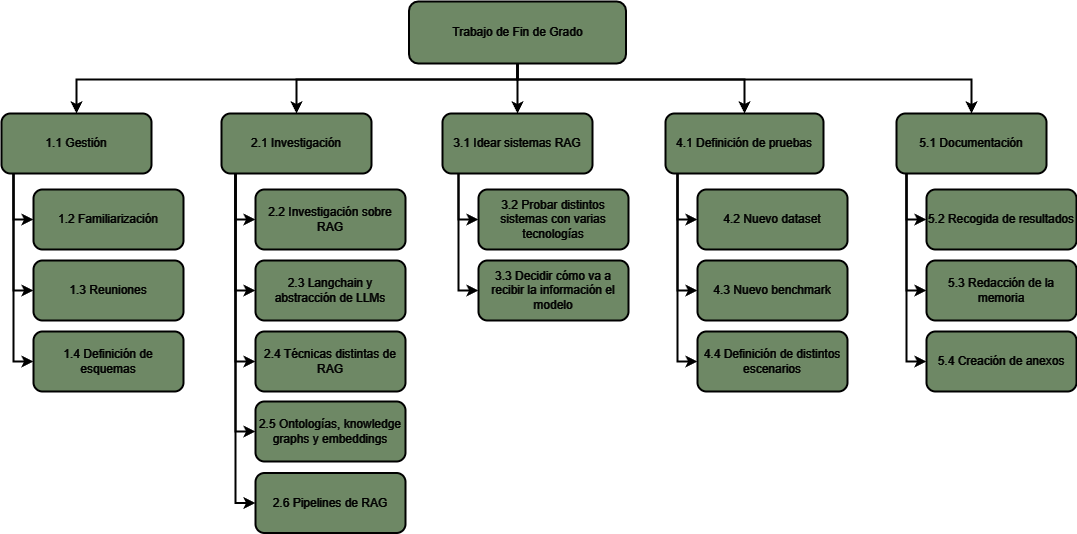
\includegraphics[width=1\textwidth]{images/tfg_edt.png}
    \caption{Esquema de división del trabajo}
    \label{fig:edt}
\end{figure}

\subsubsection{Gestión y planificación}
En esta subsección se detallan las tareas llevadas a cabo con el fin de tener una buena gestión y planificación del proyecto.

\tabla{Reuniones}{
    \textbf{Paquete de trabajo}: Gestión
}{
    \textbf{Tiempo estimado}: 15 horas
}{
    \textbf{Descripción}: Se realizaron reuniones semanales tanto con Mikel Egaña, como con Arkaitz Carbajo, además, con Unai López se hicieron también reuniones más extensas para revisar el estado del proyecto.
}{
    \textbf{Entregables}: Actas de reuniones
}{
   \textbf{Recursos}: Microsoft Teams en las reuniones telemáticas y OneNote para la toma de notas. 
}


\subsubsection{Investigación}
Esta sección del proyecto ha sido la que más tiempo ha tomado, ya que se dedicó mucho tiempo al principio a investigar sobre el estado del arte y las tecnologías a utilizar. Además, durante la fase de desarrollo también se han realizado investigaciones para mejorar el modelo.

\tabla{Investigación sobre el funcionamiento de los LLMs}{
    \textbf{Paquete de trabajo}: Investigación
}{
    \textbf{Tiempo estimado}: 20 horas
}{
    \textbf{Descripción}: Se investigó sobre el funcionamiento de los LLMs, cómo se entrenan y cómo se utilizan. Además, se investigó sobre los diferentes modelos de LLMs y cuál sería el más adecuado para el proyecto.
}{
    \textbf{Entregables}: Notas sobre el funcionamiento de los LLMs
}{
   \textbf{Recursos}: OneNote para la toma de notas 
}

\tabla{Langchain y abstracción de LLMs}{
    \textbf{Paquete de trabajo}: Investigación
}{
    \textbf{Tiempo estimado}: 20 horas
}{
    \textbf{Descripción}: Durante este paquete de trabajo de consultó un curso sobre RAG y Langchain, que se utilizó de base para implementar los sistemas de RAG que se evalúan en este trabajo.
}{
    \textbf{Entregables}: Notas sobre Langchain y abstracción de LLMs
}{
   \textbf{Recursos}: ChatGPT and LangChain: The Complete Developer's Masterclass~\cite{udemy}
}

\tabla{Técnicas de RAG}{
    \textbf{Paquete de trabajo}: Investigación
}{
    \textbf{Tiempo estimado}: 20 horas
}{
    \textbf{Descripción}: Se investigó sobre el estado del arte de sistemas de RAG y sobre cómo son utilizados en la actualidad. Además, se investigaron técnicas de recuperación de información con distintas bases de conocimiento.
}{
    \textbf{Entregables}: Notas sobre técnicas de RAG
}{
   \textbf{Recursos}: OneNote para la toma de notas 
}

\tabla{Ontologías, knowledge graphs y embeddings}{
    \textbf{Paquete de trabajo}: Investigación
}{
    \textbf{Tiempo estimado}: 30 horas
}{
    \textbf{Descripción}: Se investigó sobre ontologías y knowledge graphs, que se consultaron también en las reuniones con Mikel Egaña. Además, se investigaron embeddings y se hicieron pruebas para determinar qué información era útil para recuperar de una base de datos vectorial. Además, se probaron distintas bases de datos vectoriales.
}{
    \textbf{Entregables}: Notas sobre ontologías, knowledge graphs y embeddings. Decisión en base de datos vectorial.
}{
   \textbf{Recursos}: OneNote para la toma de notas. Visual Studio Code para la programación
}

\tabla{Pipelines de RAG}{
    \textbf{Paquete de trabajo}: Investigación
}{
    \textbf{Tiempo estimado}: 20 horas
}{
    \textbf{Descripción}: Se investigó sobre creación de pipelines con RAG, recuperando información de una base de conocimiento para máyor precisión generando JQL. Se probó a introducir en el benchmark el pipeline.
}{
    \textbf{Entregables}: Notas sobre RAG. Código con distintas pruebas.
}{
   \textbf{Recursos}: OneNote para la toma de notas. Visual Studio Code para la programación
}


\subsubsection{Ideas sistemas RAG}

\subsubsection{Definición de pruebas}
Durante esta sección se definieron las pruebas que se iban a realizar para evaluar la calidad de cada una de las alternativas. Se ideó un nuevo conjunto de datos y se modificó el código del benchmark para ajustarlo al pipeline de RAG y permitir que sea replicable.

\tabla{Creación de nuevo Dataset}{
    \textbf{Paquete de trabajo}: Definición de pruebas
}{
    \textbf{Tiempo estimado}: 2 horas
}{
    \textbf{Descripción}: Se creó un nuevo conjunto de datos con 100 preguntas, que se utilizó para evaluar las distintas alternativas propuestas. Además, se utilizó un dataset existente en Hugging Face~\cite{datasetHF} para complementar el conjunto de datos.
}{
    \textbf{Entregables}: Nuevo conjunto de datos, archivo CSV.
}{
   \textbf{Recursos}: Visual Studio Code para la programación
}

\tabla{Modificación del benchmark}{
    \textbf{Paquete de trabajo}: Definición de pruebas
}{
    \textbf{Tiempo estimado}: 5 horas
}{
    \textbf{Descripción}: Se modificó el código del benchmark para ajustarlo al pipeline de RAG y permitir que sea replicable. Se añadieron las pruebas con el nuevo conjunto de datos y se realizaron pruebas con el nuevo conjunto de datos.
}{
    \textbf{Entregables}: Código modificado del benchmark
}{
   \textbf{Recursos}: Visual Studio Code para la programación
}
